% iaus2esa.tex -- sample pages for Proceedings IAU Symposium document class
% (based on v1.0 cca2esam.tex)
% v1.04 released 17 May 2004 by TechBooks
%% small changes and additions made by KAvdH/IAU 4 June 2004
% Copyright (2004) International Astronomical Union

\NeedsTeXFormat{LaTeX2e}

\documentclass{iau_FM}
\usepackage{graphicx}

\title[FM 10 ~~The Hosts of Stellar Explosions - Resolving the Site of the Explosion ] %% give here short title %%
{Local environments of SNe Ic and Ic-BL}

\author[Selsing et al.]   %% give here short author list %%
{Jonatan Selsing$^1$, Lise Christensen$^1$, Christina Th{\"o}ne$^2$ 
%%  \thanks{Present address: Fluid Mech Inc., 24 The Street, Lagos, Nigeria.},
 \and Maryam Modjaz$^3$}

\affiliation{
$^1$Dark Cosmology Centre, Niels Bohr Institute, University of Copenhagen, \\ 
Juliane Maries Vej 30, 2100 Copenhagen O, Denmark \\ email: {\tt jselsing@dark-cosmology.dk, lise@dark-cosmology.dk} \\[\affilskip]
$^2$Instituto de Astrofisica de Andalucia, \\

 Glorieta de la Astronomia s/n, 18008 Granada, Spain \\email: {\tt christina.thoene@gmail.com} \\ 
 
$^3$Center for Cosmology and Particle Physics, New York University \\
Meyer Hall of Physics, 4 Washington Place, room 529, New York, NY 10003 \\email: {\tt christina.thoene@gmail.com}}

\pubyear{2015}
\setcounter{page}{1}
\jname{Astronomy in Focus, Volume 1} 
\editors{Piero Benvenuti, ed.}


\begin{document}

\maketitle

\begin{abstract}
We have observed the local explosion environments of a sample Type Ic and Type Ic-BL Supernove (SNe) selected from both targeted and non-targeted surveys using VLT/VIMOS in IFU-mode. 
 It is believed that by probing the local surroundings of the parent stellar populations of these types of SNe, valuable information can be gained about the physical conditions, which affect the type of SNe produced. The different kinds of SNe produced are determined by the initial mass and metallicity of the stellar progenitor, as well as by the metallicity-dependent mass loss in the stellar winds at the end phase of their evolution and the interaction with a sufficiently close companion star.
 
% 
%Using spatially resolved spectroscopy, we investigate the stellar progenitor populations to find statistical differences between environments belonging to the different subtypes of the most heavility envelope-stripped SNe. 
%




\keywords{nuclear reactions, nucleosynthesis, abundances, (stars:) supernovae: general}

\end{abstract}




\firstsection % if your document starts with a section,
              % remove some space above using this command.
\section{Project}


At the redshift of the galaxies we have selected, we spatially resolve regions approx. 250 pc across, comparable to the size of HII regions in local galaxies and using strong nebular emission lines as a proxy for the metal content of the stellar population, we can investigate if the conditions for the two types of SNe differ. The connection between long-duration gamma-ray bursts (GRBs) and broad-lined SNe Ic and the existence of SNe Ic-bl without observed GRBs raises the question of what distinguishes a GRB progenitor from that of an ordinary SN Ic-bl without a GRB, and this project will help with the elucidation of this. Moreover, from the HII region ages and stellar mass estimates, we examine the two suggested progenitor models for stripped SNe: single massive Wolf-Rayet (WR) stars with main-sequence masses of larger than 30 solar masses that have experienced mass loss during the main sequence and WR stages, vs. binaries from lower-mass He stars.

To answers this, we have taken data for 19 SN Ic and Ic-BL hosts using the IFU
installed at VLT/VIMOS which gives spatially resolved spectra allowing
diagnostics
to be determined locally which for the redshift of the host
corresponds to the
physical sizes of the molecular clouds hosting the stellar
progenitor
population. We show in Fig.\,\ref{fig:intro:snifu} a mosaic of the
H$\alpha$
emission determined from the VIMOS data superposed on the SDSS images
of the
host which we can translate into a star formation rate. Additionally
using
stellar population modeling, we can constrain the progenitor age and
thereby the
mass that will help discerning between the different types of
progenitor stars. 



\begin{figure}[htb]
	
	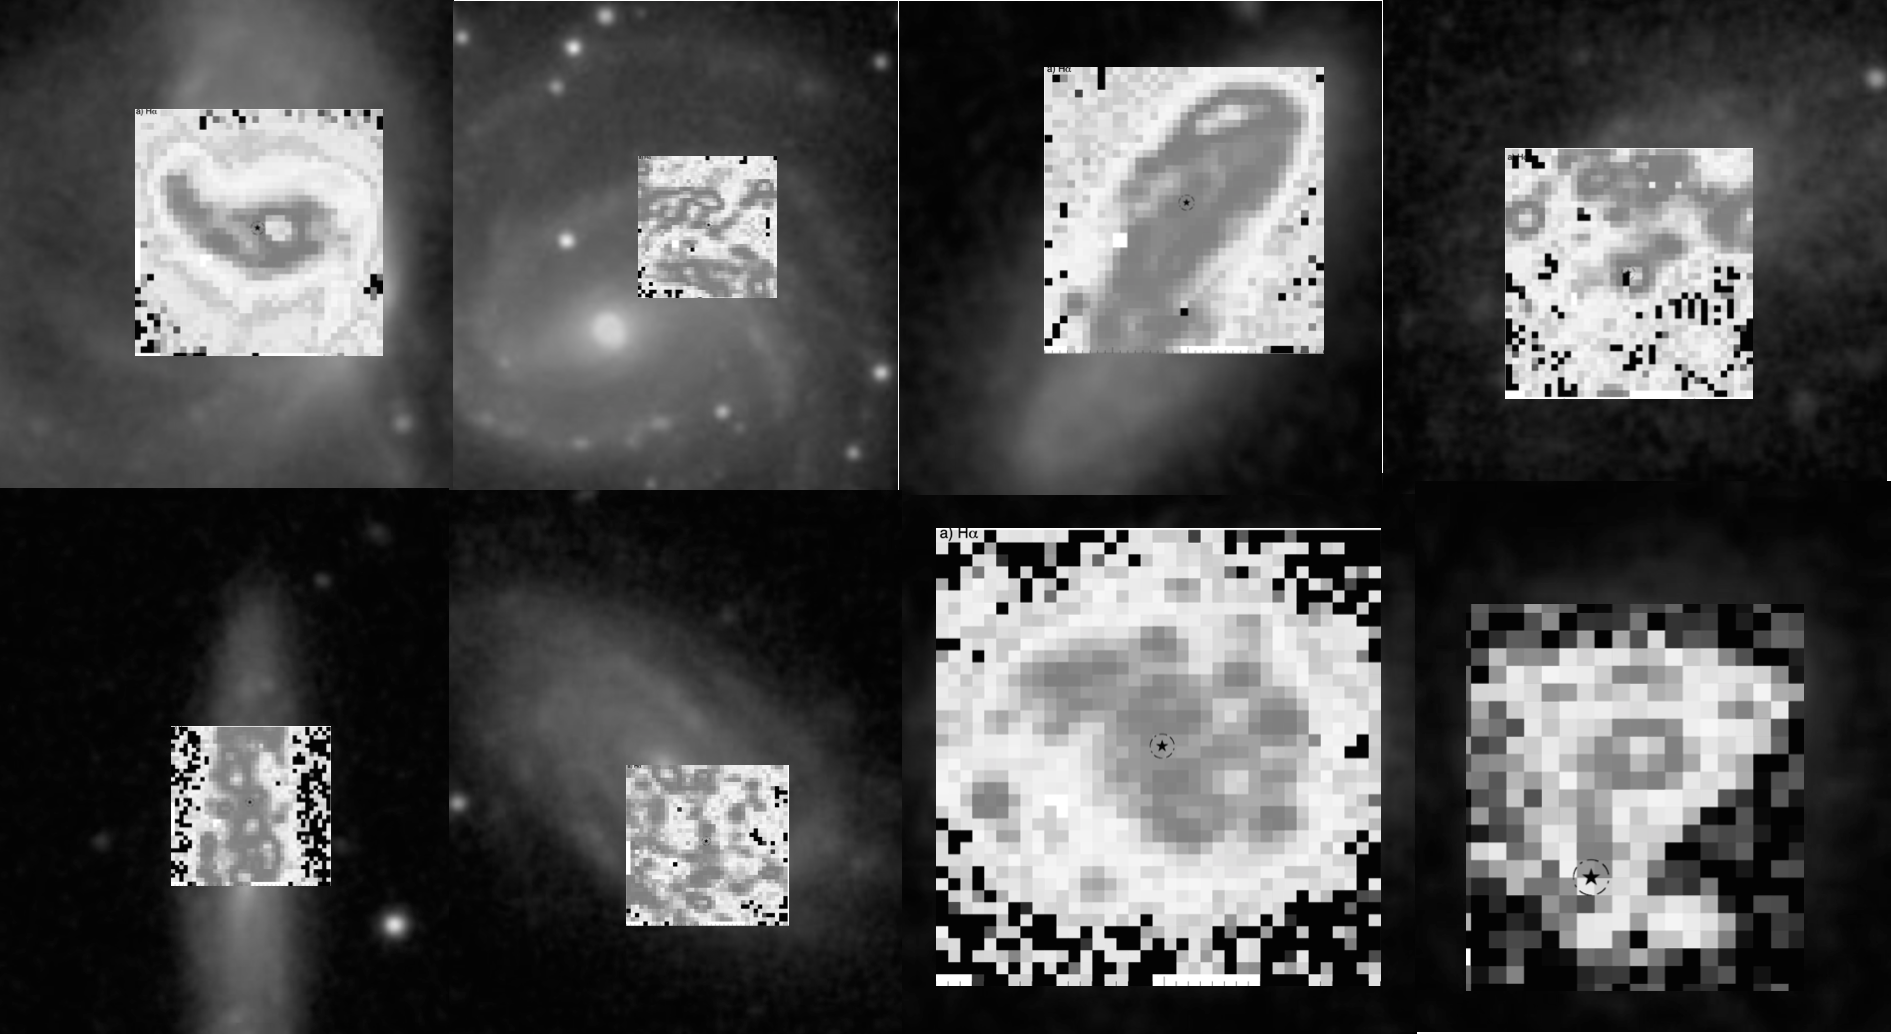
\includegraphics[width=\textwidth]{gfx/ifu}
	
	\caption{A mosaic showing 8 of the targeted SN Ic and Ic -BL host galaxies with the H$\alpha$ flux determined from the VIMOS observation superposed on the SDSS postage stamps. This is part of our sample, investigating the local properties of helium-poor SNe. }
	
	\label{fig:intro:snifu}
\end{figure}

For the metallicities determined locally we reproduce the trend seen earlier
that Ic-BL prefer lower metallicity environments as compared to normal Ic.
 This is still preliminary very work
and the values might chance slightly. A thing to note is that the 1-$\sigma$
intervals around the mean values are consistent within the errors, therefore
pointing to a non-significant difference in the types of environments preferred.





\begin{thebibliography}{}



\bibitem[(Kuncarayakti (2013))]{Kuncarayakti2013}
{Kuncarayakti et al. 2013, AJ, 146, 30}

\bibitem[(Graham \& Fruchter (2013))]{Graham2013}
{Graham, J. F. \& Fruchter, A. S. 2013, ApJ, 774, 119}


\end{thebibliography}



\end{document}
